
\documentclass[12pt, twoside]{article}

\usepackage{lingmacros}
\usepackage{tree-dvips}
\usepackage{hyperref}
\usepackage{listings}
\usepackage{graphicx}
\usepackage[T1]{fontenc}
\usepackage{tgothic}
\usepackage{tikz} 
\usepackage{titlesec}
\usepackage{amsmath}

\usetikzlibrary{positioning,chains,fit,shapes,calc}
\definecolor{myblue}{RGB}{255,255,255}
\definecolor{mygreen}{RGB}{255,255,255}

\graphicspath{ {.} }
\lstset{basicstyle=\ttfamily}

\hypersetup{
    colorlinks,
    citecolor=black,
    filecolor=black,
    linkcolor=black,
    urlcolor=black
}

% \setcounter{secnumdepth}{0}

\begin{document}

\setlength{\parindent}{0pt}
\titleformat{\paragraph}
{\normalfont\normalsize\bfseries}{\theparagraph}{1em}{}
\titlespacing*{\paragraph}
{0pt}{3.25ex plus 1ex minus .2ex}{1.5ex plus .2ex}

\begin{titlepage}
  \begin{center}
    \textbf{LICEUL TEORETIC "AVRAM IANCU"}
    
    \vspace{2cm}
    \large{\textbf{LUCRARE PENTRU OBȚINEREA COMPETENȚELOR PROFESIONALE ÎN INFORMATICĂ}}
  \end{center}
  \begin{center}
    \vspace*{\fill}
    \huge{ 
      JobShop Scheduler 
      }
    \vspace*{\fill}
  \end{center}

  \vspace{3cm}
  Profesor coordonator: \hfill Realizator:
  
  Prof Salantiu Crina   \hfill Croitoru Cristian
\end{titlepage}

\renewcommand{\contentsname}{Cuprins}
\tableofcontents
\pagebreak
\section{Introducere}

Proiectul "Job-Shop Scheduler" constă într-o aplicație
mulți-platforma care le oferă companiilor și fabricilor
o modalitate de a gestiona comenzile de produse, mașînăriile
industriale deținute și de a genera automat planuri de producție
eficiente folosind informația furnizată de ei.

\section{Limbaje, Librării și Tehnologii folosite}
Proiectul folosește două limbaje de programare, patru 
librării externe pentru cele două limbaje și diferite 
programe pentru compilarea și build-ul programului.

\subsection{Limbajul C++}
Limbajul principual al proiectului este C++, mai exact C++20.
Pentru compilare s-a folosit compilatorul GNU GCC 12.2.1.

\hypersetup{
    colorlinks=true,
    linkcolor=blue,
    filecolor=magenta,      
    urlcolor=cyan,
    pdftitle={Overleaf Example},
    pdfpagemode=FullScreen,
}

\urlstyle{same}

\subsubsection{Librării}
Am utilizat pentru salvarea fișierelor modificate de program
librăria \href{https://github.com/nlohmann/json}{JSON for Modern C++}.
\newline
Interfață grafică este scris folosind librăria 
\href{https://www.wxwidgets.org/}{wxWidgets}
, care permite crearea aplicatilor grafice
mulți-platforma(Windows, Mac, Linux).

\subsection{Limbajul Python}
Python este folosit pentru partea de vizualizare a datelor
calculate de program pentru planul de producție. Motivul pentru
care această operațiune nu este efectuată în C++ este deoarece
Python are o multitudine de librării pentru vizualizarea datelor
modelate prin structuri matematice cum ar fi vectori sau matrici.

\subsubsection{Librării}
Pentru vizualizare am folosit librăria \href{https://matplotlib.org/}{matplotlib}, care 
se ocupă cu crearea graficelor și librăria \href{https://numpy.org/}{numpy} care
permite modelarea datelor sub formă obiectelor matematice.

\subsection{Tehnologii folosite}
Fiind un proiect mare, cu mai multe fișiere sursă și cu
librării externe, am avut neovie de un Build System, adică
un program pentru a gestiona fișierele sursă și pentru a 
creea un fișier "Makefile" care e ulterior folosit în compilarea
paralelizată prin comandă "make" pe Linux și echivalentele ei
din alte sisteme de operare. \newline
Am decis să folosesc \href{https://premake.github.io/}{Premake},
un build system cu o interfață ușoară printr-un script LUA.
\subsubsection{Build Script}

\begin{lstlisting}[language={[5.0]Lua},breaklines,frame={single}]
dofile "use_wxwidgets.lua"

workspace "Atestat"
    configurations { "Debug", "Release" }

project "Atestat"
    kind "WindowedApp"
    language "C++"
    targetdir "bin/%{cfg.buildcfg}"

    files { "**.h", "**.c", "**.hpp", "**.cpp" }
    wx_config {Unicode="yes", Version="3.2", Libs="core,aui,gl"}
    filter "configurations:Debug"
      defines { "DEBUG" }
      symbols "On"

    filter "configurations:Release"
      defines { "NDEBUG" }
      optimize "On"
\end{lstlisting}

\section{Structura Proiectului}
\subsection{Structura folderelor}
Proiectul este structurat în mai multe foldere, fiecare
cu un scop diferit descris mai jos. Mai jos se află o poză
cu folderele proiectului:
\newline
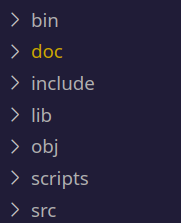
\includegraphics{folders.png}
\newline
Folderele "doc", "obj" și "lib" nu sunt explicate, deoarece
acestea conțîn codul care generează documentația prezența,
obiecte generate în procesul compilării și fișiere pentru 
link dinamic nefolosit de proiect deoarece ele se află
într-un folder extern.

\subsection{Fișierele neclasificate}
Fișierele care au un rol diferit de orice folder, astfel
neputând fi conținute de niciunul. Aceste fișier sunt:
\newline
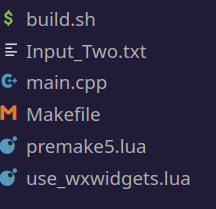
\includegraphics{neclass.png}
\newline
Pe scurt, rolurile lor sunt:
\begin{itemize}
  \item build\.sh -- un mic script bash pentru compilarea paralelizată a programului.
  \item Input\_Two.txt -- fișierul de intrare pe care este testat programul.
  \item main.cpp -- fișierul principal care conține codul de inițializare grafică.
  \item Makefile -- fișierul generat de build system pentru compilarea programului.
  \item premake5.lua -- configurarea proiectului.
  \item use\_wxwidgets.lua -- script LUA pentru a include ușor librăria externă wxWidgets.
\end{itemize}

\subsection{Folderul "src"}

Folderul "src" conține toate definițiile
claselor și funcțiilor proiectului, acestea sunt compilate în
fișiere de tip ".o" care sunt ulterior link-uite
împreună pentru a ajunge la executabilă finală.
Fișierele din folderul "src":
\newline
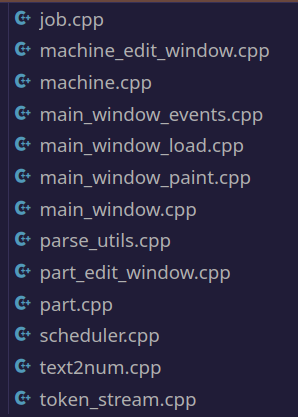
\includegraphics[scale=0.6]{sources.png}
\newline

\subsection{Folderul "include"}

Folderul "include" conține toate declararile claselor și
funcțiilor proiectului. Mai mult, conține și un fisiser
header a librăriei JSON for Modern C++, numit
"json.hpp". Acest fișier este special, deoarece conține
definiția și declararea tuturor claselor și funcțiilor din
librărie, fără a fi nevoie de linking dinamic.

\subsubsection{Subfolderul "gui"}

Subfolderul "gui" conține declarări ale claselor legate
de interfață grafică.

\subsubsection{Subfolderul "text2num"}

Subfolderul "text2num" conține declararile funcțiilor
din librăria scrisă de mine numită "text2num", librărie
care face conversia de la numere scrise în cuvinte, la
valoarea lor corespunzătoare că număr scris în cifre.
\newline
\newline
Fișierele din folderul "include":
\newline
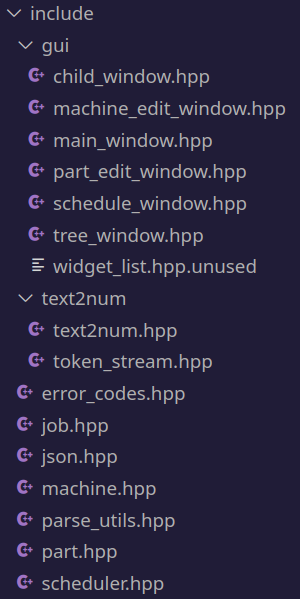
\includegraphics[scale=0.6]{include.png}
\newline

\subsection{Folderul "bin"}
Folderul "bin" conține executabilele proiectului
adică rezultatele procesului de build. Este structurat
în două subfoldere: "Debug" pentru executabilele cu
simboluri de depanare și "Release" pentru executabilele
compilate cu opțiunea de optimizare și fără simboluri
de depanare.

\subsection{Folderul "scripts"}
Folderul "scripts" conține codul scris în Python,
acest cod se ocupă cu vizualizarea calculelor făcute
de programul principal C++. Motivul pentru care am ales
acest stil de arhitectură este pentru a permite clienților
să utilizeze proprile moduri de vizualizare a datelor.

\section{Parsare}

O bună parte a codului proiectului se ocupă
de partea de parsare a fișierelor utilizatorului.
Motivul pentru care această funcționalitate are
așa mare importantă este pentru a facilita migrarea
companiilor mici, fără infrastructură digitală, la
această aplicație. Programul oferă două metode de parsare:
\begin{itemize}
  \item Parsarea Fuzzy
  \item Parsarea JSON
\end{itemize}

\subsection{Parsarea Fuzzy}
Parsarea Fuzzy permite utilizatorului să facă greșeli
în denumirile unei masinairi, de exemplu, dacă acesta
scrie "Fierăstrău Automat" prima dată iar mai apoi greșește
și scrie "Ferăstrău Atutomat", programul va face legătură
între cele două și va folosi formularea corectă. Totuși
această metodă nu este corectă în proporție de 100\% și poate
da greși.

\subsubsection{Mașînă de stare}
% \tikzset{block/.style={rectangle,draw,minimum height=2cm,minimum width=2cm}}
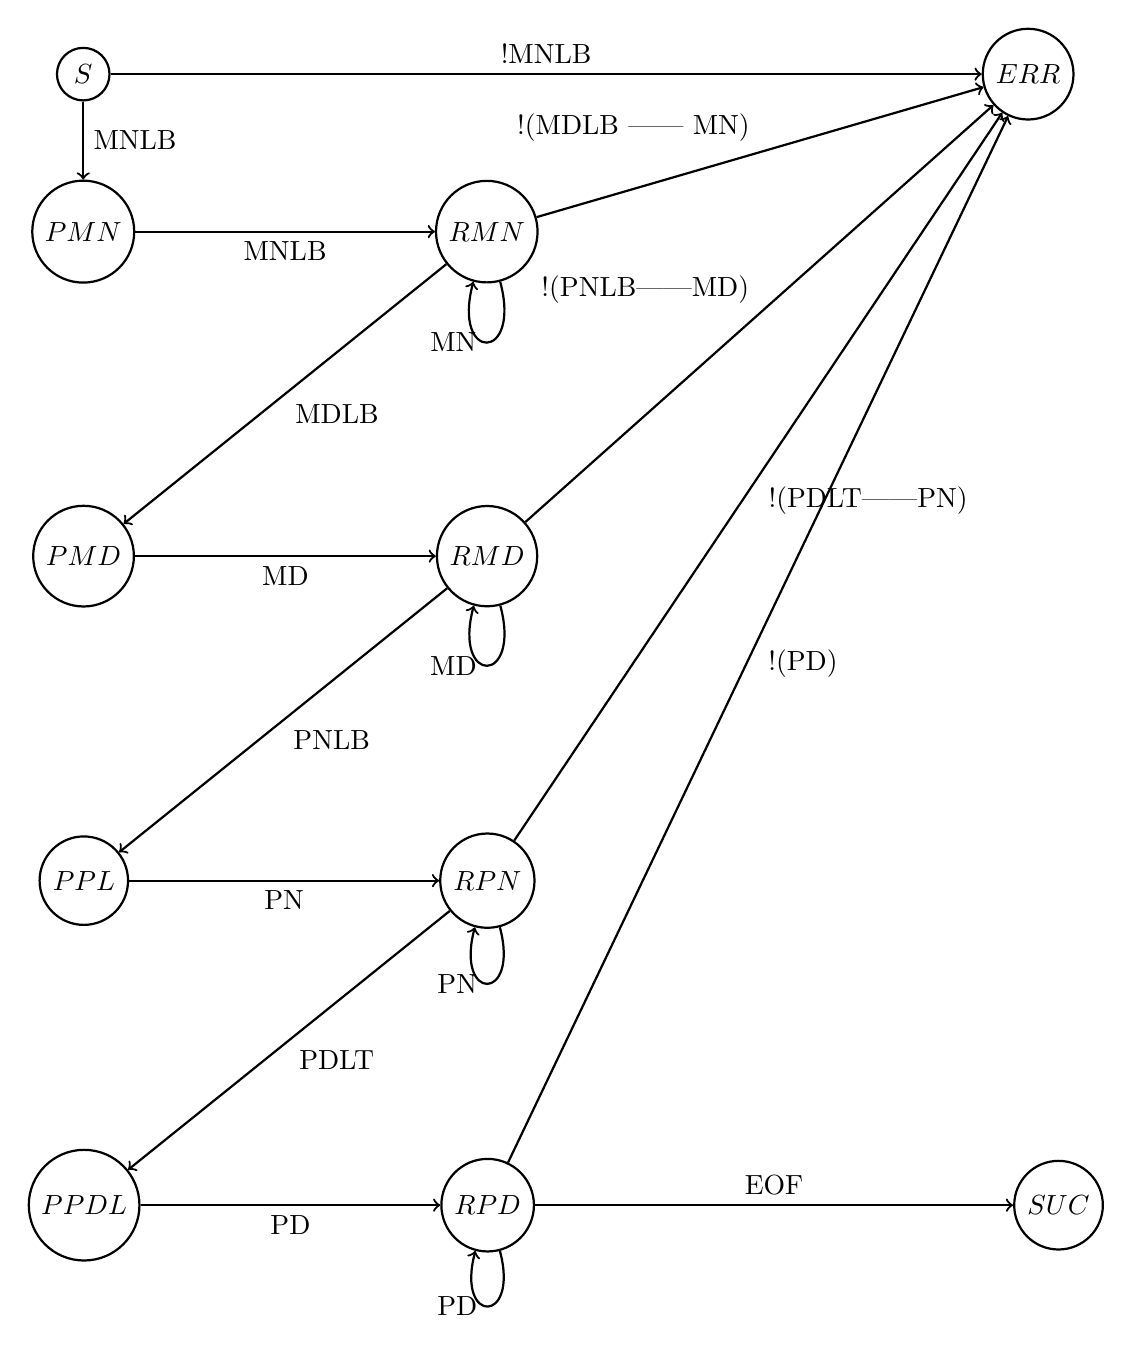
\begin{tikzpicture}[node distance={30mm}, thick, main/.style = {draw, circle},align=center] 
  \node[main] (1) {$S$}; 
  \node[main] (-1)[left of=1,xshift=15cm] {$ERR$}; 
  \node[main] (2) [below of=1,yshift=1cm] {$PMN$}; 
  \node[main] (3) [right of=2,xshift=2.125cm] {$RMN$}; 
  \node[main] (4) [below left of=2,xshift=2.125cm,yshift=-2cm] {$PMD$}; 
  \node[main] (5) [right of=4,xshift=2.125cm,yshift=0cm] {$RMD$}; 
  \node[main] (6) [below left of=4,xshift=2.125cm,yshift=-2cm] {$PPL$}; 
  \node[main] (7) [right of=6,xshift=2.125cm,yshift=0cm] {$RPN$}; 
  \node[main] (8) [below left of=6,xshift=2.125cm,yshift=-2cm] {$PPDL$}; 
  \node[main] (9) [right of=8,xshift=2.125cm,yshift=0cm] {$RPD$}; 
  \node[main] (10) [right of=9,xshift=4.250cm,] {$SUC$}; 


  \draw[->] (1) to node[right]{MNLB}(2); 
  \draw[->] (1) to node[above]{!MNLB}(-1); 

  % \draw[->] (2) to node[left]{MDLB}(4); 

  \draw[->] (2) to node[below]{MNLB}(3); 
  \draw[->,loop below] (3) to node[left]{MN}(3); 
  \draw[->] (3) to node[below right]{MDLB}(4); 
  \draw[->] (3) to node[above left]{!(MDLB || MN)}(-1);

  \draw[->] (4) to node[below]{MD}(5); 
  \draw[->,loop below] (5) to node[left]{MD}(5); 
  \draw[->] (5) to node[below right]{PNLB}(6);
  \draw[->] (5) to node[above left]{!(PNLB||MD)}(-1); 
    
  \draw[->] (6) to node[below]{PN}(7); 
  \draw[->,loop below] (7) to node[left]{PN}(7); 
  \draw[->] (7) to node[below right]{PDLT}(8);
  \draw[->] (7) to node[below right]{!(PDLT||PN)}(-1); 

  \draw[->] (8) to node[below]{PD}(9); 
  \draw[->,loop below] (9) to node[left]{PD}(9); 
  \draw[->, below] (9) to node[above]{EOF}(10); 
  % \draw[->] (9) to node[below right]{PNLB}(8);
  \draw[->] (9) to node[below right]{!(PD)}(-1); 

\end{tikzpicture} 

\subsubsection{Legendă mașînă de stadiu}
Stări:
\begin{itemize}
  \item S - Stare de start, verifică dacă e valid documentul.
  \item PMN -- Stare care așteaptă simbolul pentru
              lista de nume și ID-uri userspace
              ale mașînăriilor.
  \item RMN -- Stare în care se parsează numele și ID-ul
              userspace al unei mașînării, până la simbolul
              pentru lista de descrieri ale mașînăriilor.
  \item PMD -- Stare care așteaptă și se verifică simbolul 
              pentru lista de descriereile mașînăriilor.
  \item RMD -- Stare în care se parsează descriereile mașînăriilor.
  \item PPL -- Stare în care se așteaptă și verifică simbolul pentru
              lista de nume is ID-uri userspace ale părților
              care trebuie produse.
  \item RPN -- Stare în care se parsează numele și ID-ul părților.
  \item PPDL-- Stare în care se așteaptă și verifică simbolul
                care denotă ineperea listei de descrieri ale procesului
                de fabricare al unei părți.
  \item RPD -- Stare în care se parsează descrierea procesului de
              fabricare al unei părți.
  \item ERR -- Stare de ieșire, eroare la parsare.
  \item SUC -- Stare de ieșire, document parsat cu succes.
\end{itemize}
Condiții de tranziție:
\begin{itemize}
  \item MNLB -- Simbol de început al listei numelor și ID-urilor userspace al mașînăriilor.
  \item MN -- Simbol pereche UserspaceID.Nume
  \item MDLB -- Simbol de început al listei descrierilor mașînăriilor.
  \item MD -- Simbol care desemnează descrierea unei mașînării.
  \item PNLB -- Simbol de început al listei numelor și ID-urilor userspace al părților.
  \item PN -- Simbol pereche UserspaceID.NumeParte
  \item PDLT -- Simbol de început al listei descrierilor părților.
  \item PD -- Simbol care desemnează descrierea unei părți.
  \item EOF -- Simbol care desemnează sfârșitul unui fișier.
\end{itemize}


\setcounter{secnumdepth}{4}


\subsubsection{Descriere detaliată}

Fiecare stare din diagramă 4.1.1 are o implementare complexă
și diferită. Arhitectură de parsare este una simplă și 
șablonată, urmărind un șablon liniar de parcurgere a stărilor.

\paragraph{Starea de început (S)}

Starea de început va aștepta simbolul \textbf{availablemachines}
pe care îl obține din începutul unui fișier de intrare fuzzy, adică
\textbf{Available machines:}. Pentru a evita riscul unei parsari
eșuate, verificarea utilizează o funcție care transformă simbolul
scris de om, în unul ușor de verficat, exemplu fiind $\textbf{Available machines:}
\Rightarrow \textbf{availablemachines}$. Codul funcției este următorul:

\begin{lstlisting}[language={C++},breaklines,frame={single}]
bool is_machine_list_begin(std::string& line){
    conv_to_parsable(line);
    return line.find("availablemachines") != std::string::npos;
}
\end{lstlisting}

\pagebreak
\begin{lstlisting}[language={C++},breaklines,frame={single}]
void conv_to_parsable(std::string& line){
    std::string new_str;
    std::transform( line.begin(), line.end(),
                    line.begin(),tolower);

    for(auto & c : line){
        if(isalnum(c))
            new_str.push_back(c);
    }
    line = new_str;
}
\end{lstlisting}

\paragraph{Parsarea ID și Nume (PMN și RMN)}

Parsarea ID și Nume se face după detectarea simbolului
MNLB, prin citirea unei linii, extragerea primului număr
până la întâlnirea unui caracter ne-numeric, extragerea apoi
a primelor cuvinte până la întâlnirea unor caractere care nu
aparțîn alfabelului englez sau nu sunt \textbf{\_ sau -}.
Codul verificării este următorul:

\begin{lstlisting}[language={C++},breaklines,frame={single}]
int parse_machine(std::string& line, Job* job){
    auto id = extract_first_num(line);
    auto m_name = extract_first_words(line,[](char c){
        return isspace(c) || isalpha(c) || c=='-' || c=='_';
    });

    if(!has_chars(m_name)) return ERROR_BAD_NAME;
    
    while(isspace(m_name.back()))
        m_name.pop_back();

    for(auto & existing_machine : job->machines){
        if(id == existing_machine.get_id()){
            return ERROR_ID_EXISTS;
        }
    }

    Machine mach(m_name,id);
    job->machines.push_back(mach);
    return 1;
}
\end{lstlisting}

\paragraph{Parsarea descrierilor mașînăriilor(PMD și RMD)}
Starea această este inițiată de simbolul \textbf{machinefeatures}.
\break
\break

Parsarea descrierilor mașînăriilor este un procedeu delicat
deoarece necesită că linia care specifică cooldown-ul să fie
succesoare și direct sub linia care specifică capacitatea
mașînăriei. Acesta este un lucru care, în viitor, poate fi
îmbunătățit pentru a nu prezența o astfel de contrangere
majoră. 
\break
\break

Comparativ cu parsarea de până acum, această stare citește
câte două linii deoadata și verifică dacă prima este cea de
capacitate iar a două de cooldown, emițând o eroare în cazul
în care această cerință nu este îndeplinită. Parsarea unei
caracteristici urmează următorul algoritm:
\begin{enumerate}
  \item Din linia capacității, extrage ID-ul userspace al mașînăriei descrise.
  \item Extrage de pe ambele linii textul care urmează ID-ul. începe după întâlnirea simbolului
  \item Transformă în numere utilizabile de algoritm capacitatea respectiv cooldown-ul.
\end{enumerate}
\break
\break

Ultimul pas al algoritmului este complex, parsarea fiind fuzzy,
permite că numărul care definește capacitatea și cooldown-ul
să fie scris cu cifre (1029) sau cu litere, în limba engleză
(one thousand twenty nine), algoritmul folosindu-se de funcția
\textbf{text2num} care poate parsa ambele cazuri în întregi pe
64 de biți.
\break
\break

Codul acestei stări este următorul:
\pagebreak
\begin{lstlisting}[language={C++},breaklines,frame={single}]

int parse_machine_feature(std::string& line1, std::string& line2, Job* job){
    auto machine_id = extract_first_num(line1);

    bool found_machine = false;
    for(auto & existing_machine : job->machines){
        if(machine_id == existing_machine.get_id()){
            found_machine = true;
        }
    }
    if(!found_machine) return ERROR_BAD_ID;

    std::string cap_str = extract_last_words(line1);
    std::string cool_str = extract_last_words(line2);

    std::size_t capacity = text2num(cap_str);
    std::size_t cooldown = text2num(cool_str);

    for(auto & existing_machine : job->machines){
        if(machine_id == existing_machine.get_id()){
            existing_machine.set_capacity(capacity);
            existing_machine.set_cooldown(cooldown);
        }
    }

    return 1;
}
\end{lstlisting}

\paragraph{Parsarea părților (PPL, RPN, PPDL și RPD)}

Parsarea părților este implementată asemănător cu cea
a mașînăriilor, singură diferența fiind la parsarea
descrierilor, unde pot există un număr arbitrar de linii pentru
o descriere, ceea ce a necesitat un algoritm mai bun, care
consumă linii până detectează că a ajuns la o altă descriere
moment în care se oprește din consumat și parsează descrierea.

\subsubsection{Funcția text2num}

Funcția \textbf{text2num} este o funcție care primește că
parametru un string care e reprezentarea în cuvinte a unui
număr mai mic de $2^{60}$ și returnează un întreg cu semn de
64 de biți egal cu numărul reprezentat de string. Funcția nu
are rată de succes 100\% dacă numărul introdus nu urmează
regulile de gramatică din limba engleză. Mai mult, pentru
scopurile programului, funcția interpretează orice string
care nu conține un număr că $0$ și ia că prioritate cifrele
din parametru înainte cuvintelor. De exemplu stringul 
\textbf{"120 five thousant forty five"} este $120$ nu $5045$.

\vspace{1cm}
Algoritmul din spatele funcției este următorul:
\begin{enumerate}
  \item Verifică dacă există numere în parametru
  \item Dacă există, formează un număr cu acele numere
  \item Daca nu exista, interpretează parametrul.
\end{enumerate}
% \vspace{1cm}
Algoritmul de interpretare este următorul:
\begin{enumerate}
  \item Sparge parametrul în tokenuri predefinite.
  \item Transforma tokenurile în întregi.
  \item Parcurge șirul de întregi.
  \item Daca următorul întreg este mai mic decât cel curent atunci adaugă la număr, altfel înmulțește.
\end{enumerate}


De exemplu, stringul \textbf{"five thousand forty five"}
devine șirul de întregi \textbf{{5, 1000, 40, 5}} care
reprezintă următoarea ecuație:
\begin{center}
  $5 \cdot 1000 + 40 + 5 = 5045$
\end{center}

\subsection{Parsarea JSON}
Parsarea JSON facilitateaza siguranță datelor citite, deoarece
în formatul JSON sunt salvate planurile de producție
citite de Parsarea Fuzzy, după eventuala lor modificare
în cazul erorilor.


Parsarea JSON este implementata folosind o librărie externa
și nu necesita explcatii indetaliu. Formatul JSON este un
format standardizat și folosit peste tot în industrie.
Un exemplu mic de obiect JSON este:

\begin{lstlisting}[frame={single}]
{
  "nume":"Catalin Stefan Ion",
  "varsta":47,
  "masina":null
}
\end{lstlisting}

\section{Modelarea Datelor}
Proiectul conține trei clase principale folosite
pentru modelarea datelor. Aceastea sunt \textbf{Job},
\textbf{Machine} și \textbf{Part}. Raționamentul din
spatele acestei alegeri este structura fișierului de
intrare și problema rezolvata de program.


Structura fișierului este următoarea:
\begin{lstlisting}[frame={single}]
Available machines:
1. Band saw
2. Lathe
3. Knee Mill
4. Part washer
5. Dual-spindle machining center
6. Rotary tumbler

Machine features:
1:  - Capacity: one part at a time
    - Cooldown time: none

2:  - Capacity: one part at a time
    - Cooldown time: none

3:  - Capacity: one part at a time
    - Cooldown time: none

4:  - Capacity: one part at a time
    - Cooldown time: 600 seconds after each part

5:  - Capacity: two parts at a time
    - Cooldown time: none

6:  - Capacity: no limit
    - Cooldown time: none

Part list:
1. Door knob - 6 items
2. Pen - 12 items
3. Keyboard frame - 1 item
4. Intake manifold - 4 items

Part operations:
1:  - Band saw: 150 seconds
    - Lathe: 1200 seconds
    - Part washer: 100 seconds

2:  - Band saw: 50 seconds
    - Lathe: 2000 seconds
    - Knee Milll: 1200 seconds
    - Rotary tumbler: 600 seconds
    - Part washer: 200 seconds

3:  - Band saw: 200 seconds
    - Dual-spindle machining center: 8000 seconds
    - Rotary tumbler: 600 seconds
    - Parts washer: 600 seconds

4:  - Band saw: 2000 seconds
    - Knee mill: 4000 seconds
    - Dual-spindle machining center: 3000 seconds
    - Rotary tumber: 3500 seconds
    - Part washer: 1200 seconds
\end{lstlisting}


Se observa că fișierul oferă informații despre mașinării
și parti, adică clasele \textbf{Machine} și \textbf{Part}.
Clasa de \textbf{Job} este clasa care reprezintă tot fișierul
și care de unește cele doua clase mai mici.

\subsection{Clasa Part}

Clasa \textbf{Part} reprezintă o parte care trebuie produsa.
Aceastea are că membrii un ID și un nume împreună cu metode
de tip getter și setter aferente, procesul de fabricare
fiind retinunt într-o structura de date în clasa \textbf{Job}.


Definiția clasei este:

\begin{lstlisting}[language={C++},breaklines,frame={single}]
#ifndef PART_HGUARD
#define PART_HGUARD
#include 
#include 
#include "machine.hpp"

class Part
{
private:
    std::string name;
    std::size_t id;
public:
    Part(std::string name) : name(name) {};
    Part(std::string name, std::size_t id) : name(name), id(id) {};
    Part(/* args */);

    std::string get_name();
    std::size_t get_id();

    void set_id(std::size_t new_id);
    void set_name(const std::string& new_name);

    ~Part();
};

typedef std::pair PartOrder;

#endif
\end{lstlisting}

Clasa definește și un tip de data numit \textbf{PartOrder}
care reprezintă informația despre numărul de parti care
trebuie fabricate.

\subsection{Clasa Machine}
Clasa \textbf{Machine} reprezintă o mașinărie din fabirca.
Aceastea are că membrii un numele, un ID, capacitatea și
cooldown-ul și metodele de get și set aferente.

Definiția clasei este:

\begin{lstlisting}[language={C++},breaklines,frame={single}]
  #ifndef MACHINE_HGUARD
  #define MACHINE_HGUARD
  #include 
  
  class Machine
  {
  private:
      std::string name;
      std::size_t capacity;
      std::size_t cooldown;
      std::size_t id;
      
      bool in_use = false;    
  public:
      Machine(std::string name, std::size_t cap,
              std::size_t cooldown) : name(name),
              capacity(cap),cooldown(cooldown){};
  
      Machine(std::string name, std::size_t cap,
              std::size_t cooldown, std::size_t id) : 
              name(name), capacity(cap),cooldown(cooldown),
              id(id){};
  
      Machine(std::string name, std::size_t id):
          name(name), id(id){};
  
      std::string get_name();
      std::size_t get_capacity();
      std::size_t get_cooldown();
      std::size_t get_id();
  
      void set_name(const std::string& new_name);
      void set_capacity(std::size_t new_cap);
      void set_cooldown(std::size_t new_cool);
      void set_id(std::size_t new_id);
      
      Machine(/* args */);
      ~Machine();
  };
  
#endif
\end{lstlisting}

\subsection{Clasa Job}

Cea mai complexa dintre cele trei clase principale prin care
datele sunt modelate este clasa \textbf{Job}. Aceasta are în
compoziția ei trei structuri de date principale și un nume pentru
a putea fi identificata

\subsubsection{Structura de graf bipartit}

Clasa folosește un graf bipartit pentru a retine procesul de
fabricare a fiecărei parti.

\begin{center}
  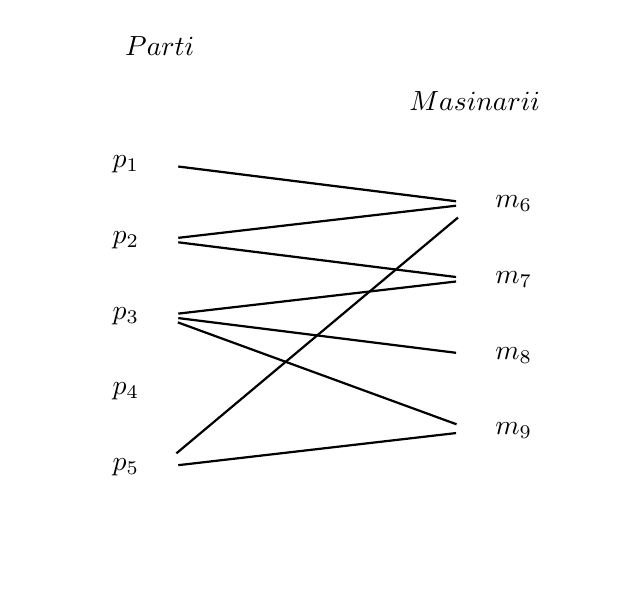
\begin{tikzpicture}[thick,
    fsnode/.style={},
    ssnode/.style={},
    every fit/.style={ellipse,draw,inner sep=5pt,text width=2cm},
    shorten >= 3pt,shorten <= 3pt
  ]

  % the vertices of U
  \begin{scope}[start chain=going below,node distance=7mm]
  \foreach \i/\xcoord/\ycoord in {1/6/8,2/5/1,3/-4/7,4/6/9,5/0/-3}
    \node[fsnode,on chain,label=left:$p_{\i}$] (f\i) {};
  \end{scope}

  % the vertices of V
  \begin{scope}[xshift=4cm,yshift=-0.5cm,start chain=going below,node distance=7mm]
  \foreach \i/\xcoord/\ycoord in {6/0/3,7/1/4,8/-2/1,9/5/9}
    \node[ssnode,on chain,label=right:$m_{\i}$] (s\i) {};
  \end{scope}

  % the set U
  \node [myblue,fit=(f1) (f5),label=above:$Parti$] {};
  % the set V
  \node [mygreen,fit=(s6) (s9),label=above:$Masinarii$] {};

  % the edges
  \draw (f1) -- (s6);
  \draw (s6) -- (f2);
  \draw (f2) -- (s7);
  \draw (s7) -- (f3);
  \draw (s8) -- (f3);
  \draw (f3) -- (s9);
  \draw (s9) -- (f5);
  \draw (f5) -- (s6);
  \end{tikzpicture}
\end{center}

Am ales acest mod de a reprezenta datele deoarece facilitateaza
implementarea ușoară a algoritmului de generare a planului de producție,
 viteza de acces și economia de memorie.
\subsubsection{Vectorii de parti și mașinării}

Clasa mai cuprinde și doi vectori care rețin părțile respectiv
mașinăriile descrise de fișierul de intrare. Am ales acest mod
de a stoca mașinările deoarece facilitateaza căutarea după mai
multe criterii sacrificând eficienta.

\subsection{Constructorii}

Clasa implementează un constructor default și unul care
primește că parametru un path spre un fișier de intrare
unde vă folosi parsarea fuzzy pentru a creeaz un obiect
din acel fișier. Mai mult, oferă funcționalitate de a se salva
și de a se încarca din fișiere json.


Definiția clasei \textbf{Job} este;

\begin{lstlisting}[language={C++},breaklines,frame={single}]
#ifndef JOB_HGUARD
#define JOB_HGUARD
#include 
#include 
#include 
#include 

#include "part.hpp"
#include "machine.hpp"
#include "error_codes.hpp"
#include "text2num/text2num.hpp"
#include "parse_utils.hpp"

#include "json.hpp"
typedef std::multimap> bipartite_graph;

class Job
{
  private:
  public:
      bipartite_graph operations; 
  
      std::vector orders;
      std::vector machines;
  
      std::string name;
    
      void add_operations(size_t id_part, size_t id_machine, float time);
  
      Machine& get_machine_by_id(std::size_t);
      PartOrder& get_order_by_id(std::size_t); 
  
      std::optional> 
      get_machine_by_name(const std::string&);
      
      std::optional> 
      get_order_by_name(const std::string&);
  
      std::string as_string();
  
      void json_load(const std::string& path);
      void json_save(const std::string& path);
  
      Job(const std::string & path_to_config);
      Job(/* args */);
      ~Job();
};
#endif
\end{lstlisting}


\section{Stocarea Datelor}

Deoarece stocarea datelor este necesara, programul se folosește
de formatul \textbf{JSON} pentru a stoca obiectele de tip
\textbf{Job}. Desi citirea lor se poate face și din fișiere
scrise și citibile de un om, stocarea se poate face doar
în fișiere \textbf{JSON} pentru a asigura corectitudinea
și viteza.


Funcția de salvare a unui obiect \textbf{Job} este:

\begin{lstlisting}[language={C++},breaklines,frame={single}]
void Job::json_save(const std::string& path){
    nlohmann::json j = {
        {"name",this->name}
    };

    j["machines"] = j.array();
    for(auto & machine : this->machines){
        nlohmann::json machine_j;
        machine_j["id"] = machine.get_id();
        machine_j["name"] = machine.get_name();
        machine_j["capacity"] = machine.get_capacity();
        machine_j["cooldown"] = machine.get_cooldown();
        j["machines"] += machine_j;
    }

    j["parts"] = j.array();
    for(auto & order : this->orders){
        auto process = this->operations.equal_range(order.first.get_id());
        nlohmann::json part_j;
        part_j["id"] = order.first.get_id();
        part_j["name"] = order.first.get_name();
        part_j["amount"] = order.second;
        part_j["process"] = j.array();
        for(auto op = process.first; op != process.second; ++op){
            nlohmann::json op_json;
            op_json["machine"] = op->second.first;
            op_json["duration"] = op->second.second;
            part_j["process"] += op_json;
        }
        j["parts"] += part_j;
    }

    std::ofstream out(path);
    out << std::setw(4) << j;
}
\end{lstlisting}


Funcția de încărcare a unui obiect \textbf{Job} este:

\begin{lstlisting}[language={C++},breaklines,frame={single}]
void Job::json_load(const std::string& path){
    std::ifstream in(path);
    nlohmann::json j;
    j = j.parse(in);

    this->machines.clear();
    this->orders.clear();
    this->operations.clear();
    
    this->name = j["name"].get();

    for(auto& mj : j["machines"]){
        Machine machine(
            mj["name"].get(),
            mj["capacity"].get(),
            mj["cooldown"].get(),
            mj["id"].get());
        this->machines.push_back(machine);
    }


    for(auto& pj : j["parts"]){
        Part part(
            pj["name"].get(),
            pj["id"].get());

        this->orders.push_back({part, pj["amount"].get()});
        for(auto& opj : pj["process"]){
            this->operations.insert(
                {
                    part.get_id(),
                    {
                        opj["machine"].get(),
                        opj["duration"].get()
                    }
                }
            );
        }
    }
}
\end{lstlisting}

\section{Interfață}

Interfață proiectului este una simpla deoarece piață tintă
este cea industriala, unde funcționalitatea este cheia și nu
aspectul.

Aceasta este implementata folosind librariea \textbf{wxWidgets}
care necesita implementarea unei anumite arhitecturi. La pornire
programul lansează un obiect de tip \textbf{App} care conține
un obiect e tip \textbf{Window}, unde funcționalitatea aplicației
este implementata prin răspunsuri la eventimente cum ar fi
click-ul, apăsarea unei taste, resizing etc.


Definiția aplicației principale este:
\begin{lstlisting}[language={C++},breaklines,frame={single}]
#ifndef MAIN_WINDOW_HGUARD
#define MAIN_WINDOW_HGUARD

#define DEBUG_PRINTS

#include 
#include 
#include 
#include 
#include 
#include 

#include 
#include 
#include 
#include 

#include "../job.hpp"
#include "part_edit_window.hpp"
#include "machine_edit_window.hpp"
#include "../scheduler.hpp"

class App : public wxApp
{
public:
    bool OnInit() override;
};
 

class MainWindow : public wxFrame
{
public:
    MainWindow();
 
private:
    std::unordered_map all_jobs;
    ChildWindow* edit_window = 0;

    wxTreeCtrl* tree;
    wxTreeItemId jobs_root;
    wxTreeItemId active_item;
    wxBoxSizer* vbox;
    Job* job = nullptr;
    
    void OnHello(wxCommandEvent& event);
    void OnExit(wxCommandEvent& event);
    void OnAbout(wxCommandEvent& event);

    void OnLoad(wxCommandEvent& event);
    void OnLoadJSON(wxCommandEvent& event);
    void OnSaveJSON(wxCommandEvent& event);
    void OnCalculate(wxCommandEvent& event);
    
    void ActivateMainWindowTools();
    void BuildWindowLayout();

    void OnSelectedTreeItem(wxTreeEvent& event);
    void OnPaintTree(wxPaintEvent& event);
    
    void PartNameCallback(wxCommandEvent& event);
    void PartAmountCallback(wxCommandEvent& event);


    void MachineNameCallback(wxCommandEvent& event);
    void MachineCooldownCallback(wxCommandEvent& event);
    void MachineCapacityCallback(wxCommandEvent& event);

    void RemoveAllChildWindows();

    wxDECLARE_EVENT_TABLE();
    
};
 
enum
{
    ID_Hello = 1,
    ID_LoadJob = 2,
    ID_Tree = 4,
    TEST_TextBox = 3,
    ID_LoadJSON = 5,
    ID_SaveJSON = 6,
    ID_Calculate = 7
};

#endif
\end{lstlisting}
\subsection{Funcționalitate}

Interfață oferă posibilitatea de a modifca caracteristicile
unei mașinării dar și a unei parti. Mai mult aceasta permite
încărcarea,salvarea și generarea planului de producție
printr-un \textbf{menu bar} sau prin scurtături de la tastatura.

\subsection{Poze}
Interfață:


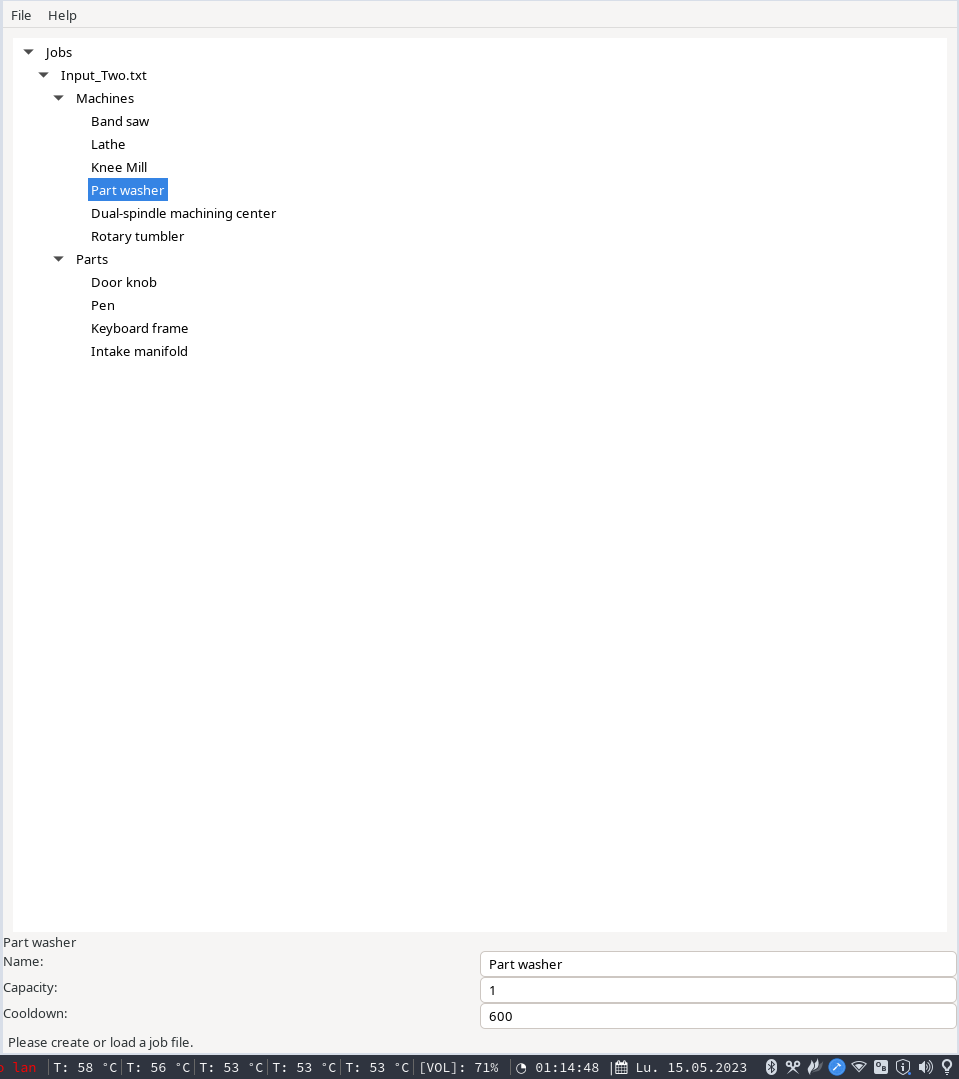
\includegraphics[scale=0.5]{interfata.png}
\section{Descrierea Problemei}

Problema este de a proiecta un software care programează
operațiunile pe piese în cel mai eficient mod posibil.
Eficiență, în acest context, se măsoară prin cât de 
repede este rulat un set de piese prin toate operațiunile
prevăzute.

\section{Îmbunătățiri pe viitor}

\subsection{Parsare}
La capitolul parasare fuzzy o valoroasa îmbunatățire ar consta
în eliminarea constrângerii că linia de capacitate și cea de cooldown
să aibă o ordine și să fie una după alta, deoarece acest lucru este
predispus la erori umane.

\subsection{Programarea operațiunilor}
Deoarece probelma propusa nu este încă rezolvata și nu exista
un algoritm polinomial pentru toate cazurile și toate constrângerile, 
singura îmbunatățire este o aproximare mai buna a programului de fabricare.

\subsection{Vizualizare}
În momentul de fata, aplicația emite un set de numere care trebuie
ulterior intrepretat de utilizator în modul în care își dorește.
O eventuala imbunatatrie este să existe funcționalitate pentru vizualizare
în moduri predefinite.

\section{Generarea planului de producție}

Algoritmul de aproximare a planului optim de producție consta
în mai mulți subalgorimti:

\begin{lstlisting}[language={C++},breaklines,frame={single}]
build_id_map();
create_dataframe();
build_time_matrix();
build_machine_queue();
build_insertion_queue();
dfs_intersection_sort();
\end{lstlisting}

\subsection{Construirea IDMap-ului}
Structura de date IDMap consta într-o structura de tip map
care servește în convertirea din ID-urile userspace ale
mașinăriilor și parților în ID-uri Algospace, adică id-uri
uniforme care încep de la $1$ și se termina la $N$ (numărul
de mașinării).

\subsection{Graful de producție}
Graful de producție este similar cu un graf orientat normal
dar consta în doua tipuri de noduri diferite.
\subsubsection{Nodul Parte}
Imaginând o pagina goala ipotetica, nodurile parte sunt
reprezentate în linie cel mai sus în pagina.
\subsubsection{Nodul Mașină}
Pe aceeași foaie, pentru fiecare ID Algospace se vă desena
orizontal un rand de mașinării cu acel ID în număr egal cu
capacitatiea mașinăriei cu ID-ul respectiv.
\subsubsection{Procesul de legare}
De la fiecare nod parte, se vă crea o muchie orientata
înspre mașinăria care urmează în pasul de producție următor.
Acolo unde deja exista o muchie, se vă adaugă încă una, existând
posibilitatea că intre doua noduri mașină să exista $M, M \le N$
miuchii.

\subsection{Construirea Dataframe-ului}
Structura de dataframe reprezintă o matrice tri-dimensionala.
Aceasta matrice servește că și o matrice de adiacenta speciala,
deoarece este necesara reprezentarea drumului fiecărei parti 
prin \textbf{graful de producție} atunci când exista posibilitatea
intersectării a doua drumuri deoarece doua mașinării au procese
de fabricare asemănătoare.

\subsection{Construirea Time Matrix-ului}
Structura de time matrix este o matrice normala cu numere reale,
de dimensiuni $M \times N$ unde $M$ este numărul de parti și $N$
numărul de mașinării. Forma generala a aceste matrici este:
\[
\begin{bmatrix}
  p_{11}+c_1 & p_{12}+c_2 &    ... &  p_{1n}+c_n \\
  p_{21}+c_1 &    ...   &    ...   &  p_{2n}+c_n \\
  ...      &    ...   &    ...   &     ... \\
  p_{m1}+c_1     &     ...   & ...   &      p_{mn}+c_n
\end{bmatrix}
\]

Unde $p_{mn}$ este timpul de fabricare a parții cu ID $m$
în mașinăria cu ID $n$ iar $c_n$ este cooldown-ul mașinăriei
cu ID $n$. Aceasta matrice permite eliminarea constrângerii
cooldown-ului mașinăriilor.

\subsection{Construirea cozilor și sortarea}

Algoritmul folosește doua cozi. Coada \textbf{MachineQueue}
reprezintă ordinea în care fiecare mașinărie procesează părțile.
Coada \textbf{IntersectionQueue} este o coada sortata care
reprezintă pentru fiecare mașinărie, partea cu cel mai scurt
timp și care începe procesul de producție pe mașinăria respectiva.
\newline
\newline
Sortarea \textbf{DFS Intersection Sort} este procedeul prin care
algoritmul aproximează planul de producție, acesta adăugând în coada
fiecărei mașinării partea cu cel mai scurt timp inițial de producție,
apoi executând un DFS pentru a adaugă partea aceea și în restul mașinăriilor
care fac parte din procesul de fabricare. Eventualele parti adăugate ulterior vor fi
adăugate astfel încât să fie minimizat timpul mort pe fiecare mașinărie.

\section{Cerințe Software și Hardware}
Cerințele necesare fiecărei librarii folosite.
\end{document} 